
%(BEGIN_QUESTION)
% Copyright 2011, Tony R. Kuphaldt, released under the Creative Commons Attribution License (v 1.0)
% This means you may do almost anything with this work of mine, so long as you give me proper credit

A ``smart'' DP transmitter with built-in square root characterization is used to measure flow through a pipe.  The orifice plate range is 0 to 125 inches WC at 0 to 277 gallons per minute:

$$\includegraphics[width=15.5cm]{i03434x01.eps}$$

A technician removes the transmitter from service and tests it by applying several air pressures to the ``H'' port while leaving the ``L'' port vented.  Here are the As-Found results:

% No blank lines allowed between lines of an \halign structure!
% I use comments (%) instead, so that TeX doesn't choke.

$$\vbox{\offinterlineskip
\halign{\strut
\vrule \quad\hfil # \ \hfil & 
\vrule \quad\hfil # \ \hfil \vrule \cr
\noalign{\hrule}
%
% Another row
{\bf Applied Pressure} ("WC) & {\bf Current signal} (mA) \cr
%
\noalign{\hrule}
%
% Another row
0 & 4.020 \cr
%
\noalign{\hrule}
%
% Another row
31.25 & 12.060 \cr
%
\noalign{\hrule}
%
% Another row
62.5 & 15.390 \cr
%
\noalign{\hrule}
%
% Another row
93.75 & 17.946 \cr
%
\noalign{\hrule}
%
% Another row
125 & 20.100 \cr
%
\noalign{\hrule}
} % End of \halign 
}$$ % End of \vbox

Calculate the largest error, in percent of (output signal) span.  Also, determine whether this looks like a zero or span error, and whether that error exists in the input (ADC) of the smart transmitter or in the output (DAC).

\underbar{file i03434}
%(END_QUESTION)





%(BEGIN_ANSWER)

This is a {\bf span} error in the output (DAC) of the smart transmitter, the greatest error being at the 100\% point (20.100 mA instead of 20.000 mA = +0.625\%). 

%(END_ANSWER)





%(BEGIN_NOTES)


%INDEX% Measurement, flow: square root characterized pressure transmitter

%(END_NOTES)

